\section{Design of \tool}

\begin{figure*}[h]
    \centering
      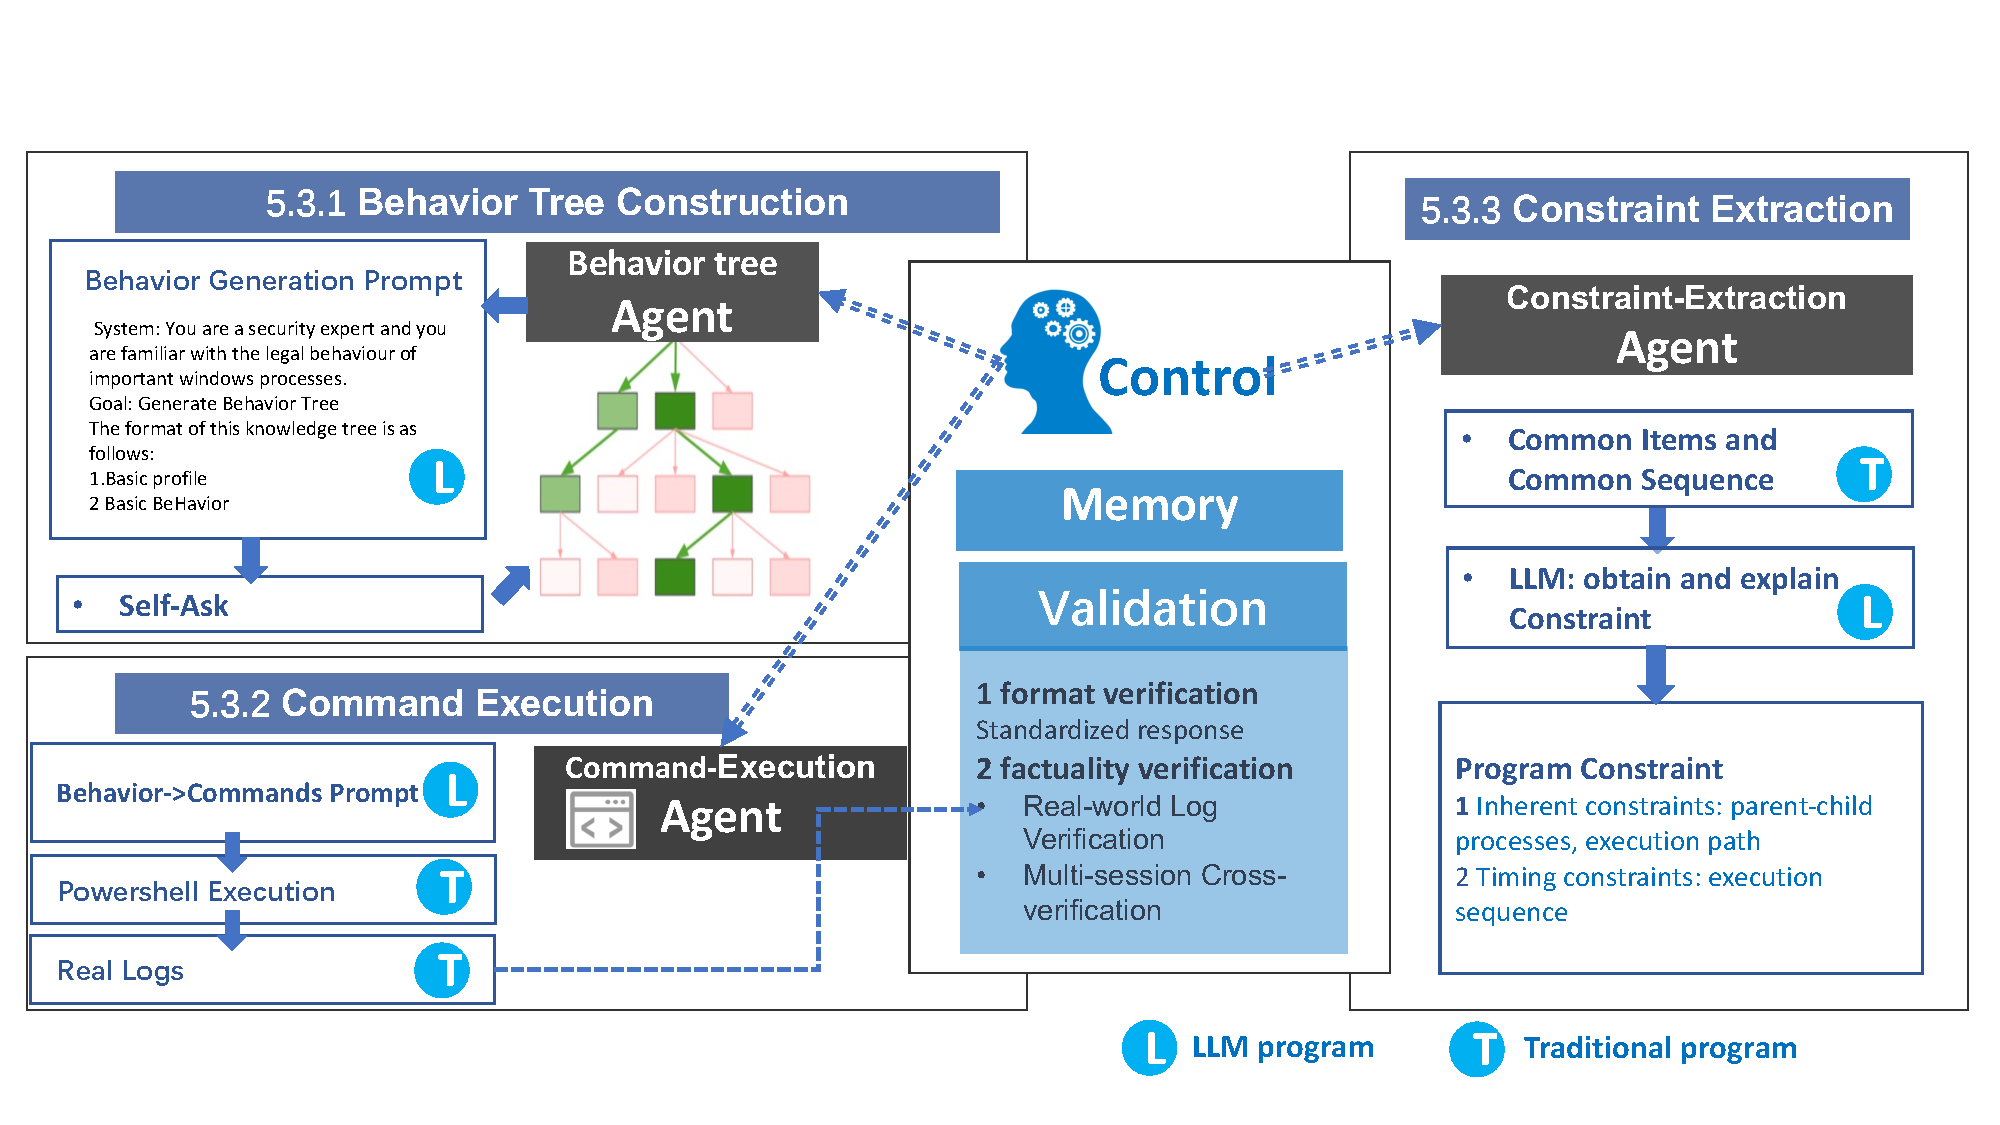
\includegraphics[width=0.9\textwidth]{figs/prompt.pdf}
    \caption{The system is controlled by a central "controller" with memory storage and validation capabilities. Our controller deploys three key modules: 1) Process Behavior Tree Construction Module, which maps out behavioral patterns; 2) Command Execution Module, which deploys active processes; and 3) Log Constraint Extraction Module, which determines log-based requirements. These units meticulously craft program profiles using LLMs-assisted strategies and traditional methods.}
    \label{fig-framework-prompt}
    \end{figure*}

\subsection{Definitions}

\subsubsection{System Entity and System Event}
We distinguish five principal entity categories: \textit{Processes}, \textit{Files}, \textit{Registry}, \textit{Dynamic Link Libraries (DLLs)}, and \textit{Network Connections}, the latter typically denoted by sockets. System entities possess unique attributes: the attributes associated with \textit{process} entities might include their Process ID (pid) or their executable paths. These entities' relationships and attributes are illustrated in Figure~\ref{fig-entity}. 

In this work, a system event $e$ is given by a tuple $\langle src, dst, rel, time\rangle$, where $src$ designates the source entity, constrained to only process entities, $dst$ indicates the target or destination entity, $rel$ denotes their interaction nature (e.g., writing into a file), and $time$ specifies the timestamp of the event occurrence.
We also illustrated the temporal relationship between events as $\langle e_1 \to e_2 \to e_3 \rangle$, indicating that the events occur in a logical sequence. 



\begin{figure}[ht]
    \centering
      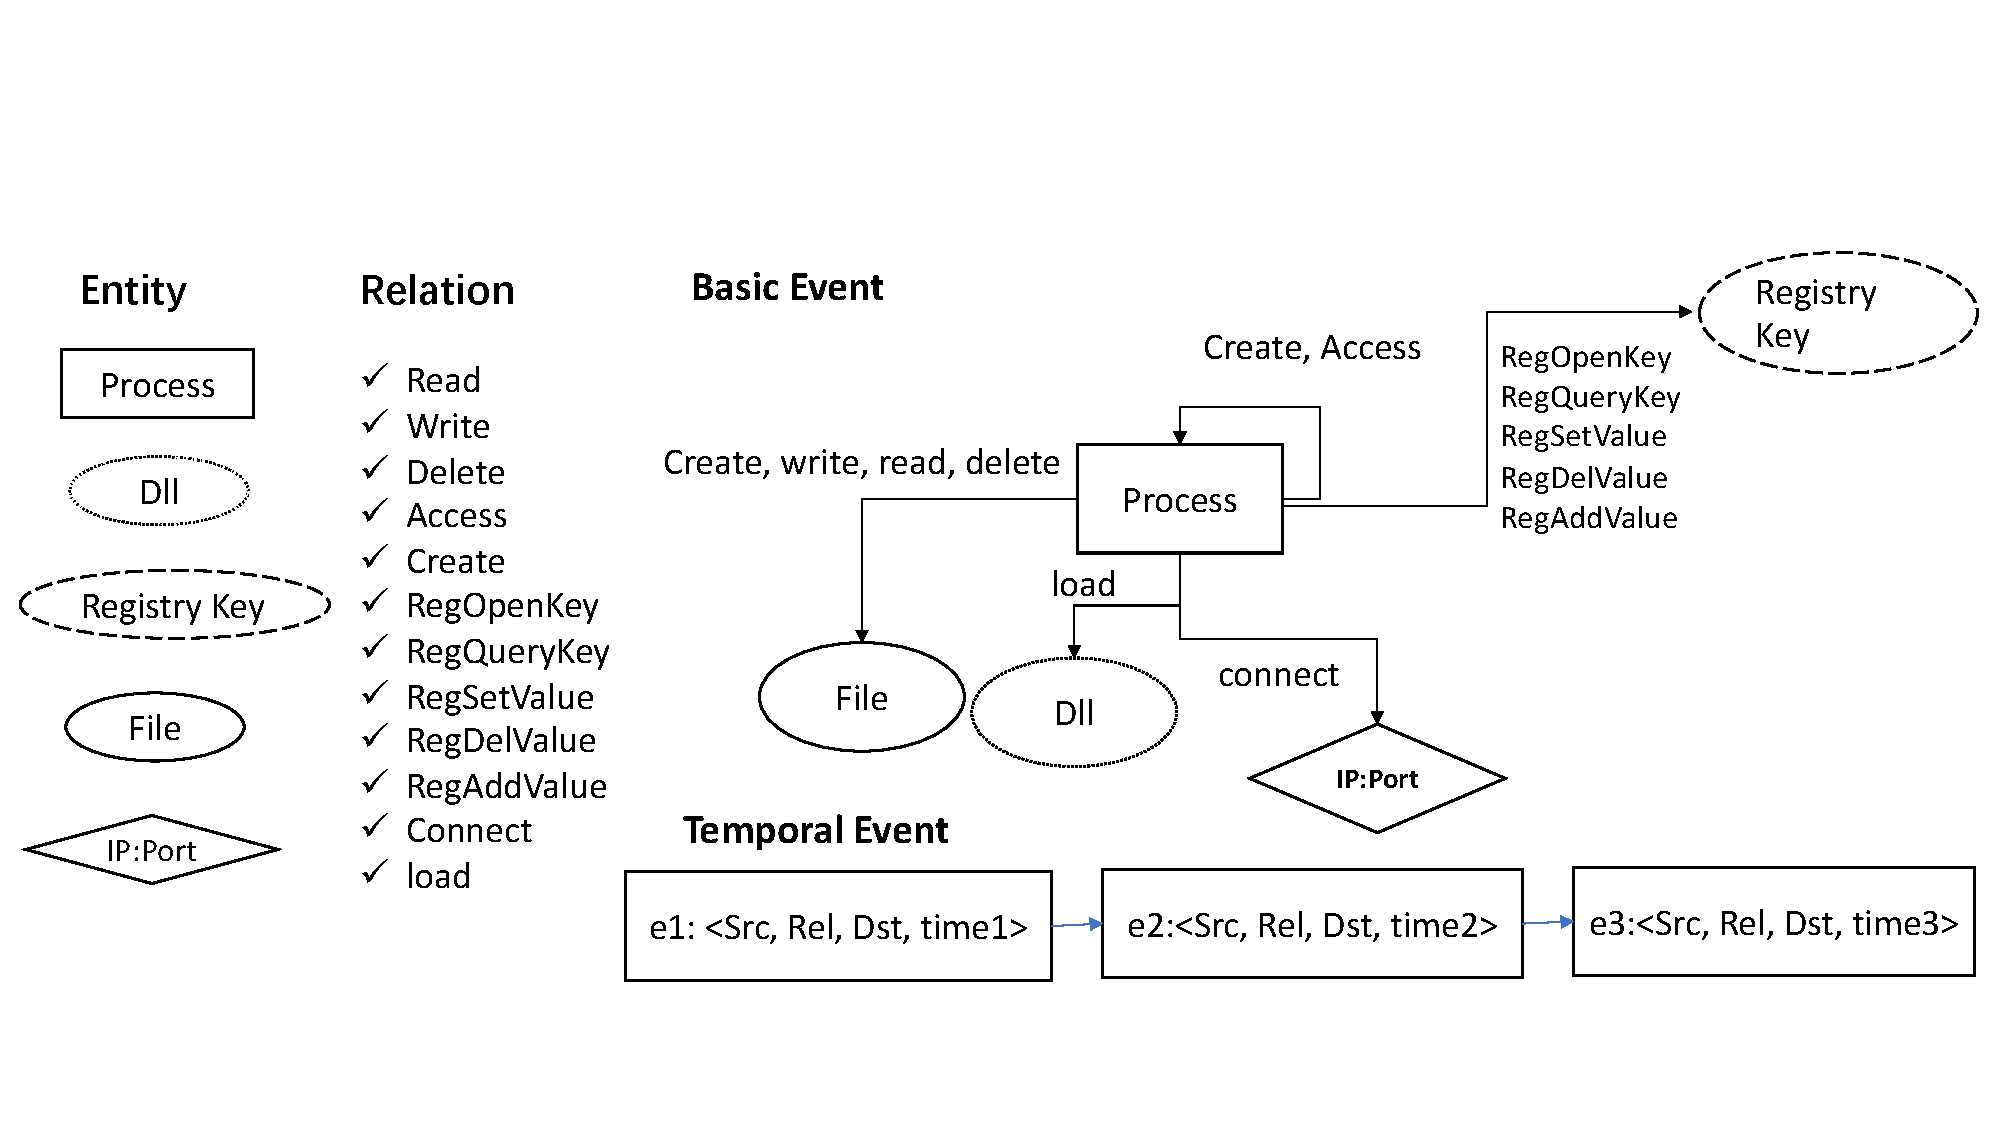
\includegraphics[width=0.45\textwidth]{figs/entity.pdf}
    \caption{System Entity and System Event.}
    \label{fig-entity}
\end{figure}

\subsection{Process Preprocessing}

\subsubsection{Process Monitoring}

Process monitoring is crucial: we need to gather logs from different processes in the system. In order to accomplish this, we use \textit{Windows}' robust log collection and processing tool, \textit{Sysmon}, to capture comprehensive system logs. \textit{Sysmon}'s default configuration ensures maximal log collection. 
However, due to the vast amount of logs, it becomes imperative to trim the data down. Using expert knowledge, we remove redundant and mundane events from the logs.

\subsubsection{Noisy Events Reduction}
Due to their inherent granularity and verbosity, audit logs introduce significant noise for analysts.
The omission of certain events does not impact the normal functioning of processes in behavioral cases. Integration of domain knowledge enhances our ability to reduce redundant events. 
To begin with, we eliminate events that repeat themselves frequently.
There are also actions that are universal to all processes, such as loading \textit{ntdll.dll}. We've streamlined these ubiquitous events for a more concise representation.

\subsubsection{Process Classification}
\label{sec:classifition}
We created a prompt to query the LLMs about whether a particular program exists by name so that classification could be completed. Using the LLMs' response, we classified these processes into three categories: legitimate process names, illegitimate process names, 
and uncertain process names (due to the LLMs database's incompleteness). Many illegitimate process names are caused by name confusion, so we can change them to legitimate process names for further evaluation.
For the legitimate and confusion processes, we use the methods described in the following sections to construct profiles. In case of illegitimate or uncertain categories, security analysts should investigate further since they may contain malware.

\subsection{Profile Construction}
\label{sec:profile_con}
Next, we present our profile building module in detail, which consists of three agent components and a central program controller.
\tool is controlled by a central program controller, which is often referred to as the "brain" of the system. In this central program controller, two components are integral: memory and validation mechanisms, which include both format and factual verification. 
Format validation of LLMs results can be solved with simple traditional programs.

In order to conduct the factual validation, multiple LLMs sessions are debating each other, as well as real-life logs being validated.
This central program controller controls three distinct agent modules: the Process Behavior Tree Construction Module, the Command Execution Module, and the Log Constraint Extraction Module. Each module manages LLMs sessions and context independently, ensuring both coherence and specialized expertise. It combines LLMs-driven processes (like behavior tree construction) with conventional computational tasks (like frequent sequence mining). A combination of traditional and LLMs-driven processes is used to create detailed process profiles under program controller guidance.

\subsubsection{Process Behavior Tree Construction}
The construction of \textit{Process Behavior Trees} is one of the most important steps in the process.
First, we define the \textit{Process Behavior Tree}.
\begin{figure}[h]
    \centering
    \begin{subfigure}{0.45\textwidth}
      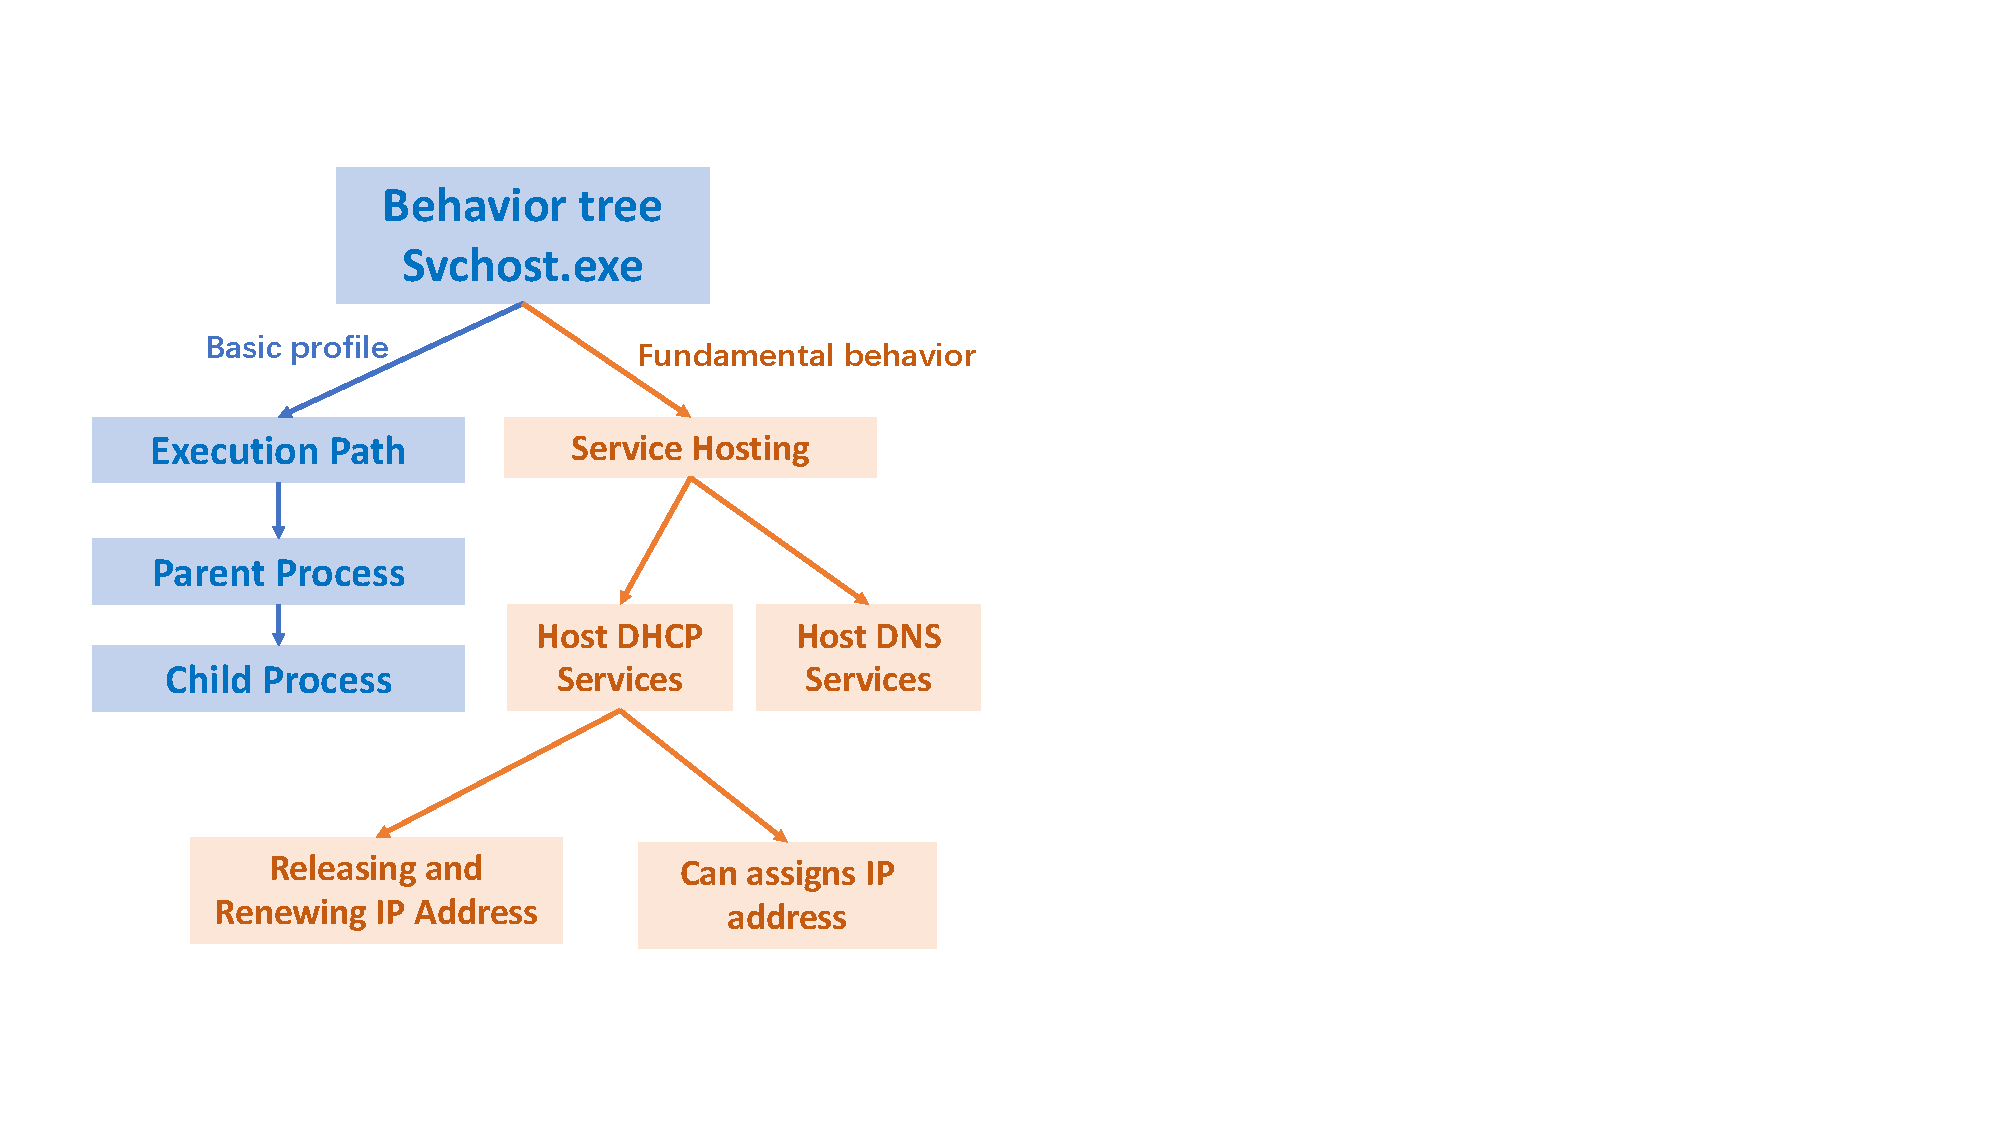
\includegraphics[width=1\textwidth]{figs/tree1.pdf}
      \caption{Process Behavior Tree Representation}
    \end{subfigure}
    \begin{subfigure}{0.45\textwidth}
    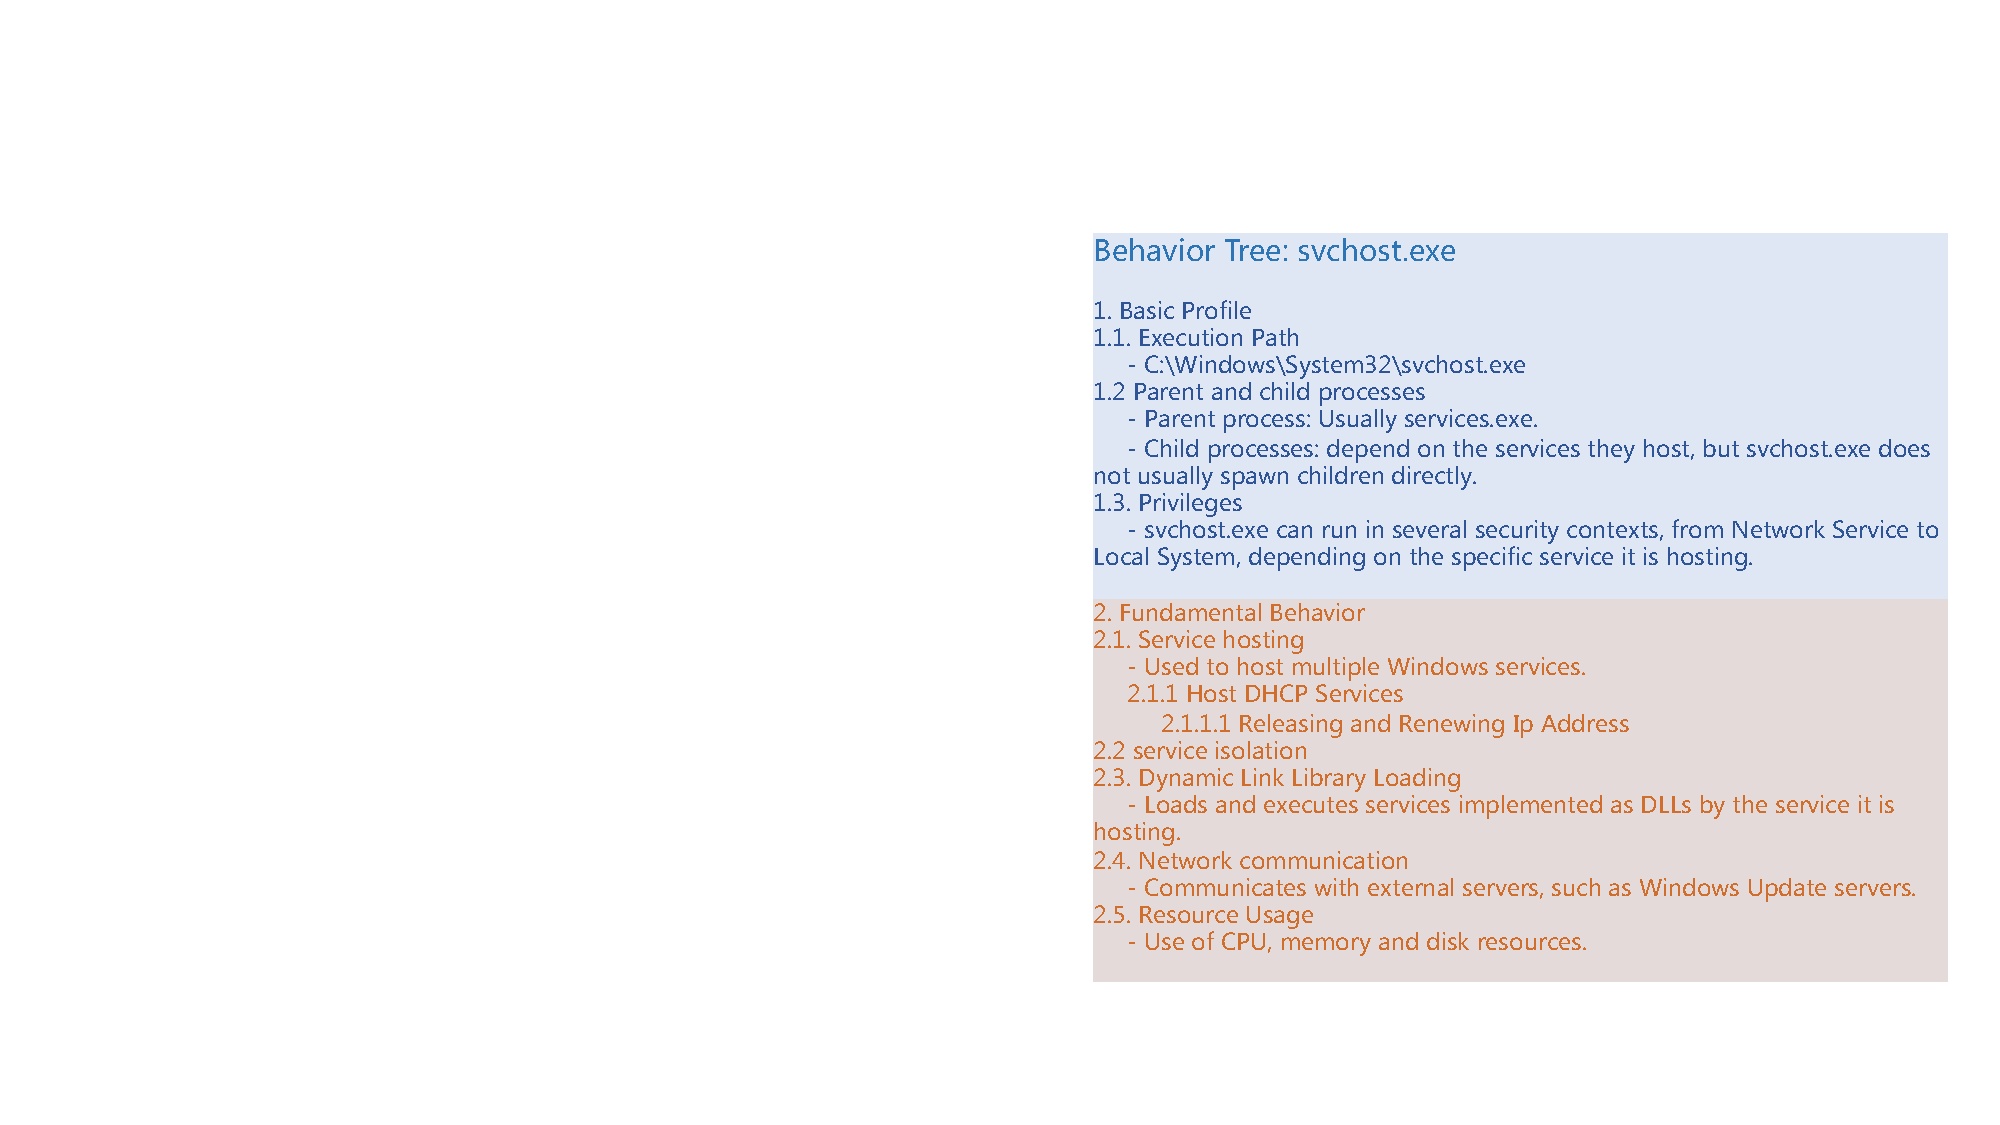
\includegraphics[width=1\textwidth]{figs/tree2.pdf}
    \caption{Process Behavior Tree Representation in natural Language}
    \end{subfigure}
    \vspace{-0.05in}
    \caption{In two formats: a) visualized tree format; and b) natural language format encoded in LLMs.}
    \label{fig:behavior-tree}
    \vspace{-0.15in}
    \end{figure}


\begin{definition}[Process Behavior Tree]
A Process Behavior Tree (BT) is a tuple \((N, B)\), where:
\begin{enumerate}
    \item \(N\) is a set of nodes organized in a tree structure. Each node represents legitimate behavior of a process. A node possesses a unique identifier within it, as well as a special node, called the root, which has no parent and does not contain any children. Except for the root of the tree, all nodes have exactly one parent and a zero number of children. There can be a sub-behavior associated with each of these children nodes.
    \item \(B\) is a function that assigns to each node \(n \in N\) a set of attributes \(B(n)\). Each attribute is a pair \((b, w)\), where \(b\) is the behavior name and \(w\) is a description or attribute of that behavior. 
\end{enumerate}
\end{definition}

To generate as many behaviors as possible, we've crafted two prompts: the \textit{Initialization Behavior Tree Prompt} and the \textit{Expansion Behavior Tree Prompt} (A detailed prompt can be found in the Appendix~\ref{prompt-init-tree}). Initially, we employ the \textit{Initialization Behavior Tree Prompt} to create a foundational behavior tree. Subsequently, this tree is expanded through iterative rounds using the \textit{Expansion Behavior Tree Prompt}. In order to create a diversity and precision of behaviors, we have incorporated four strategies:
\begin{itemize}
    \item Creating an Initial Process Behavior Tree: To ensure a standardized behavior tree, we've defined a specific output format for the behavior tree.
    \item Different Expansion Techniques in Behavior Tree Prompt: The Behavior Tree Prompt uses two distinct expansion techniques - self-ask and layer-wise. While self-ask aims at a macroscopic expansion of behaviors, layer-wise expansion delves deeper to uncover finer, detailed behaviors. To extract a comprehensive set of behaviors, these two methods combine breadth and depth searches.
    \item Using system role: LLMs often ignore earlier details in a conversation, focusing on recent interactions. As a countermeasure, we leverage the benefits of the system role and embed both roles and objectives within it.
    \item Self-Evaluation by LLMs: We aim to provide LLMs with the ability to self-criticize and review current nodes. If the LLMs determines that the branch does not require expansion, node expansion is stopped.
\end{itemize}

The resulting behavior tree is illustrated in the Figure~\ref{fig:behavior-tree}. Taking the behavior tree of \textit{svchost.exe} as an example, we begin with the basic profile. This includes details such as the execution path of the process, its parent process (the parent process of \textit{svchost.exe} can only be \textit{services.exe}), and its child processes. Following this, we have the fundamental behaviors, such as service hosting, DLL loading, and service isolation exhibited by \textit{svchost.exe}. Focusing on the most significant behavior, which is service hosting, the behavior tree can be extended to detail the specific services being hosted. From the Figure~\ref{fig:behavior-tree}, one can observe the graphical representation of the behavior tree and its expression in natural language.


\subsubsection{Command Execution}

An initial step is to design a prompt (detailed prompts can be found in Appendix:\ref{prompt-commands}) for generating commands from previous behavior trees. In order to obtain actual log files, this prompt generates corresponding system commands. We can validate some of the behaviors described in the previous step by collecting these logs. Using these logs, it is possible to directly verify some behaviors like parent processes, execution paths, and other details. It is, however, not possible to translate all system processes and behaviors into executable commands. In these cases, we employ the LLMs to produce relevant recommendations, which guide us in manually engaging with the system to obtain the required logs.

\subsubsection{Constraint Extraction}

\begin{figure*}[h]
  \begin{subfigure}{.5\textwidth}
      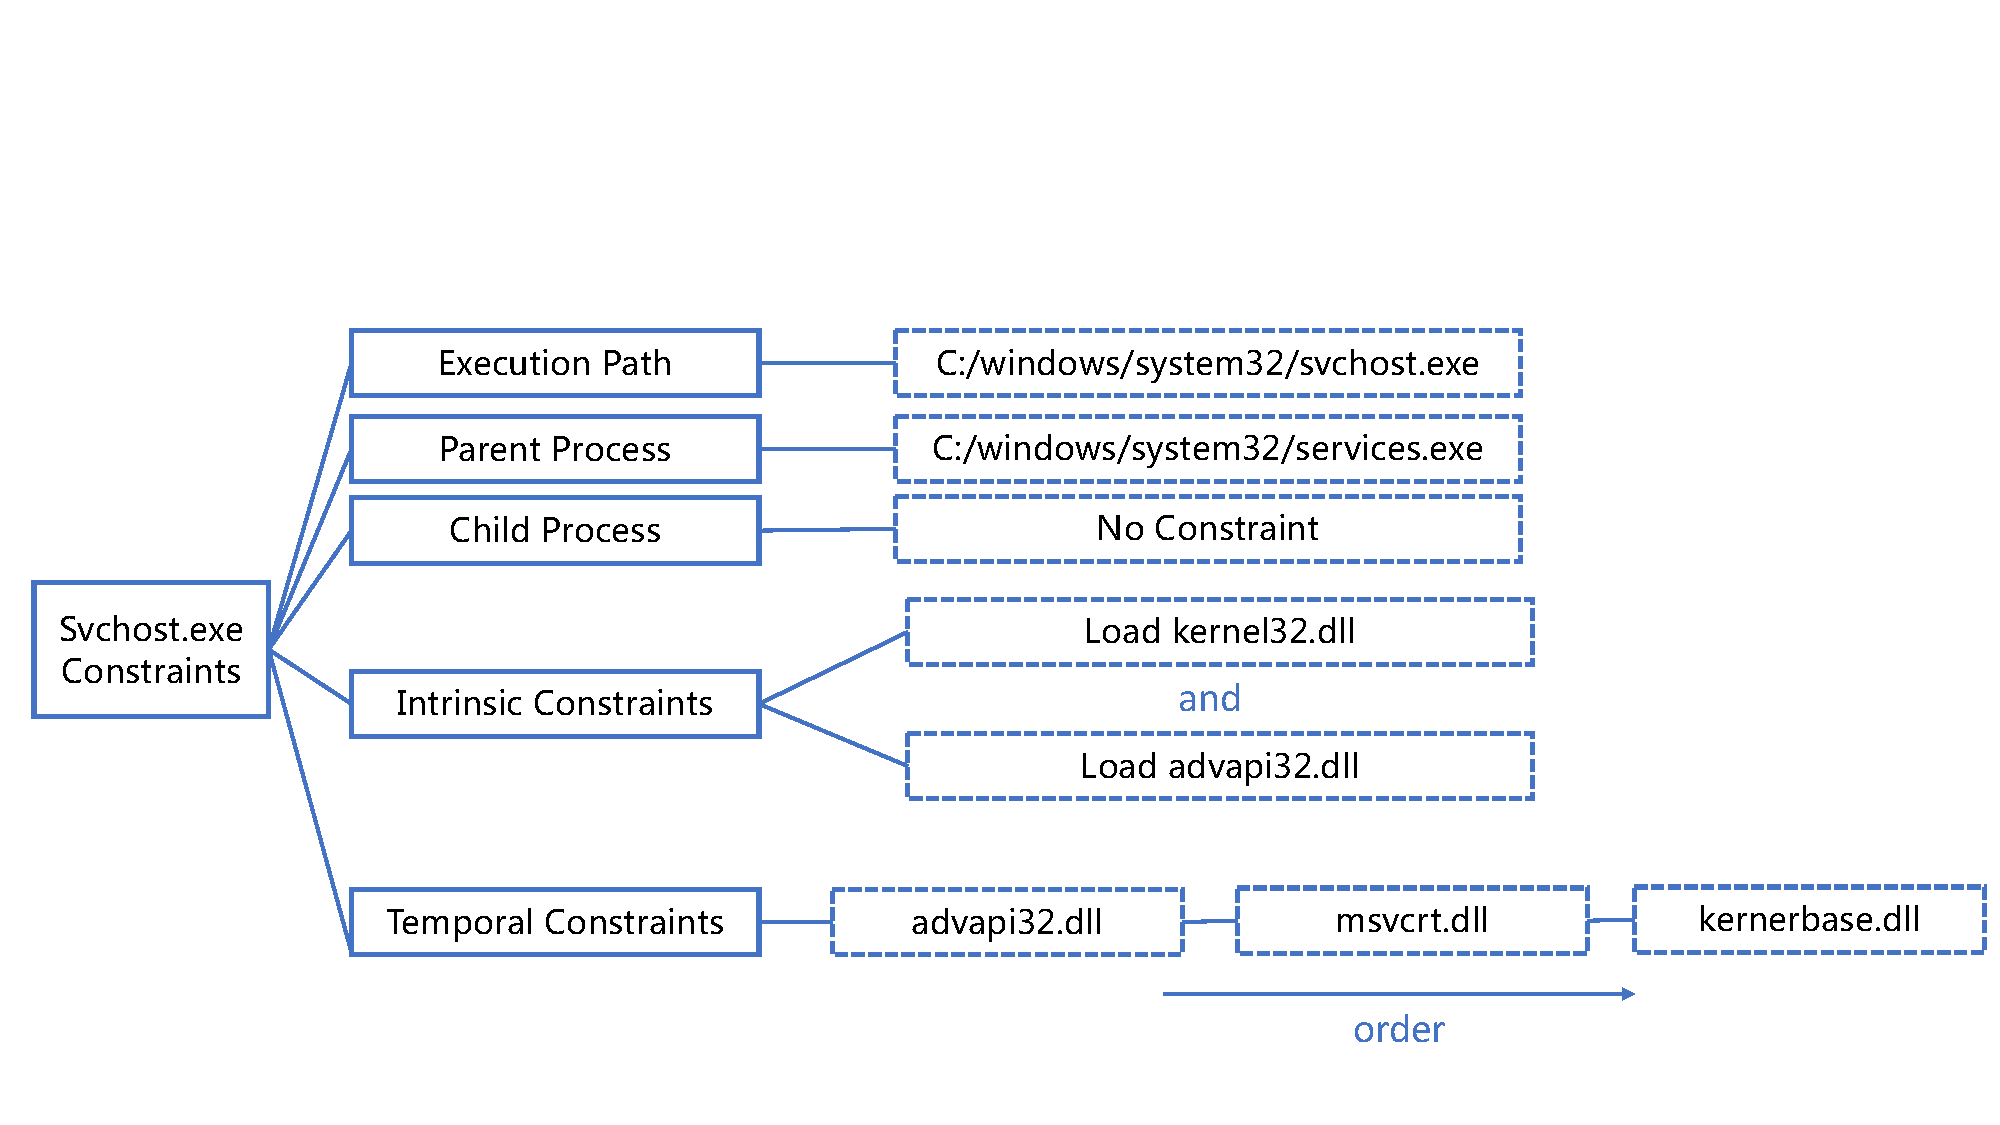
\includegraphics[width=\textwidth]{figs/svchost_constraints.pdf}
      \caption{Constraints of Svchost}
      \label{fig:cons-svchost}
  \end{subfigure}
  \hfill
  \begin{subfigure}{.5\textwidth}
      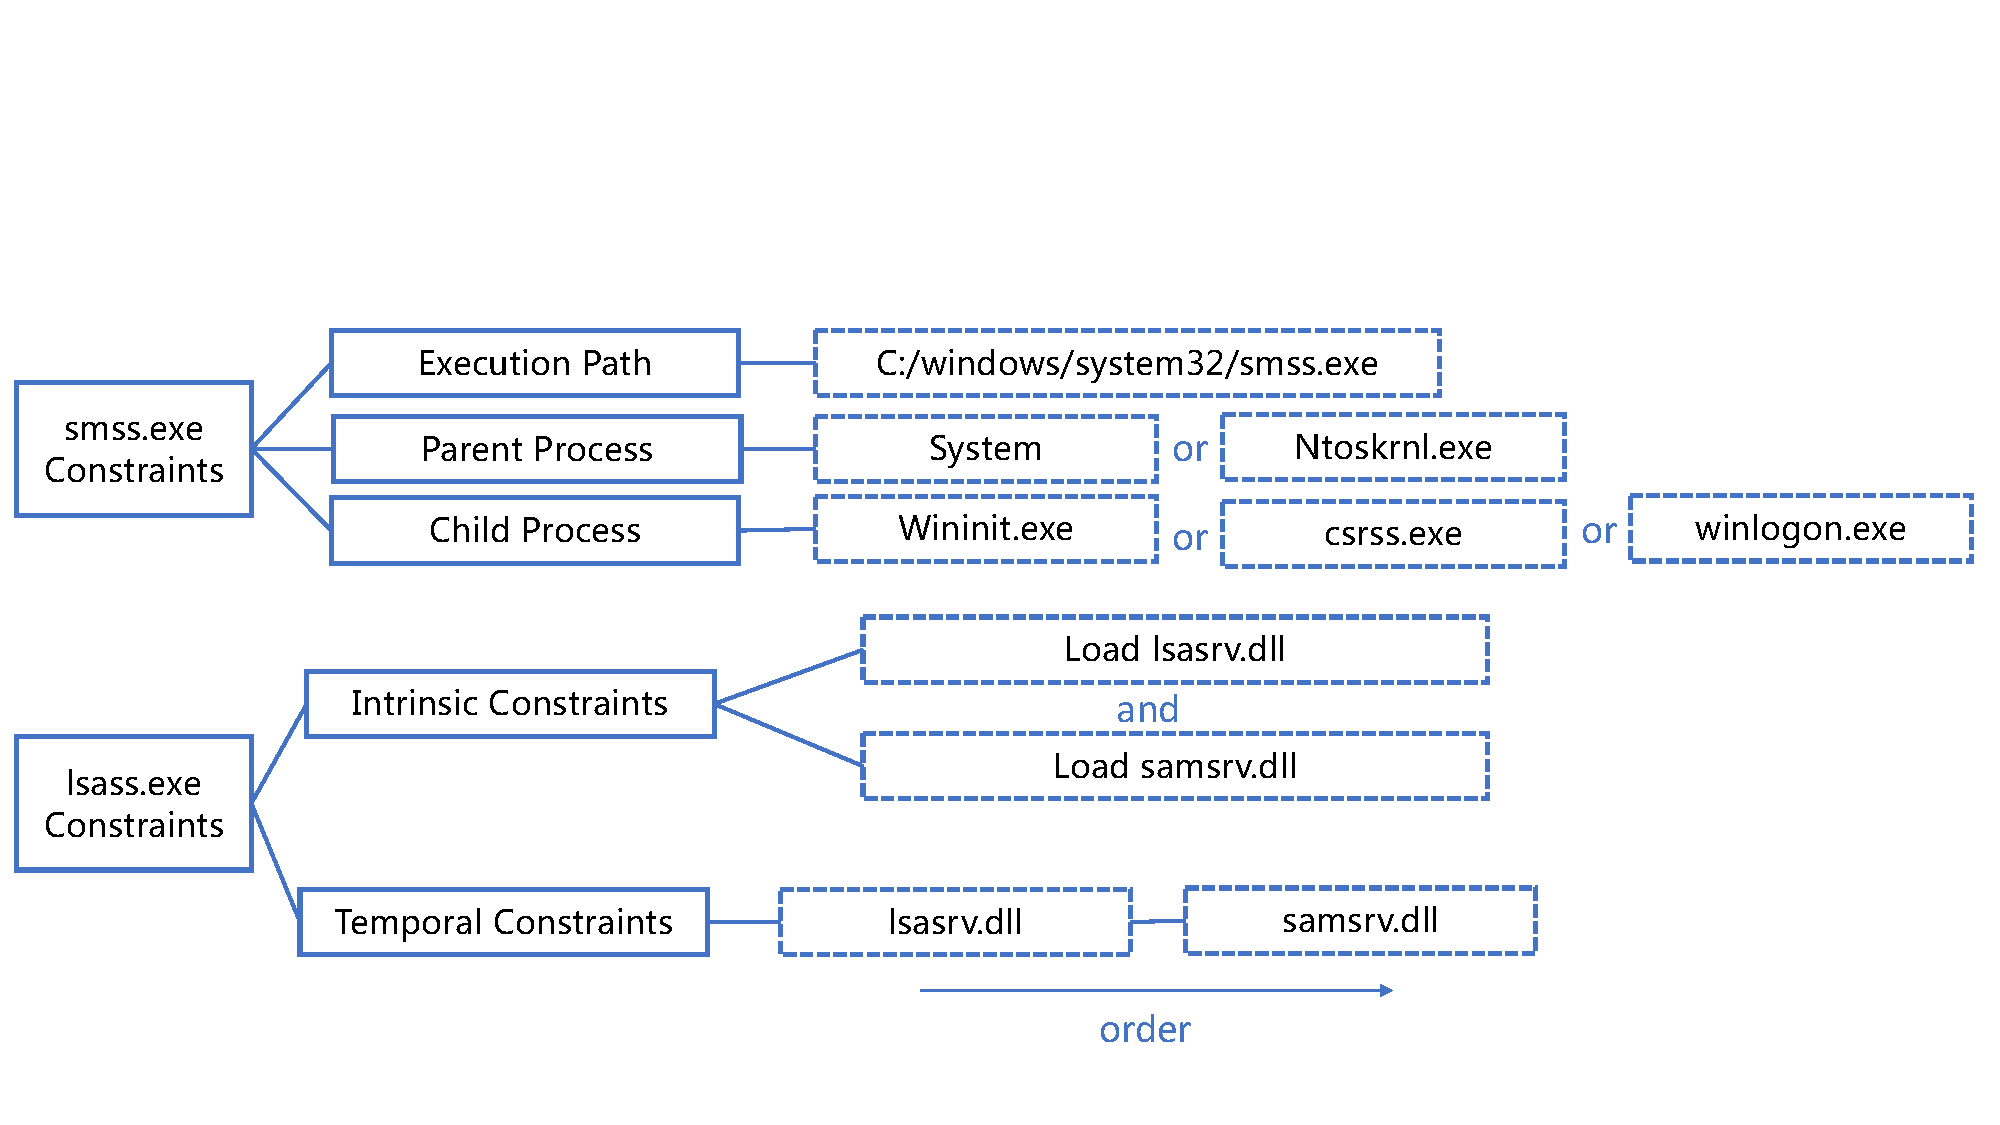
\includegraphics[width=\textwidth]{figs/smss_lsass_constraints.pdf}
      \caption{Constraints of Smss and Lsass}
      \label{fig:cons-smss-lsass}
  \end{subfigure}

  \begin{subfigure}{.5\textwidth}
      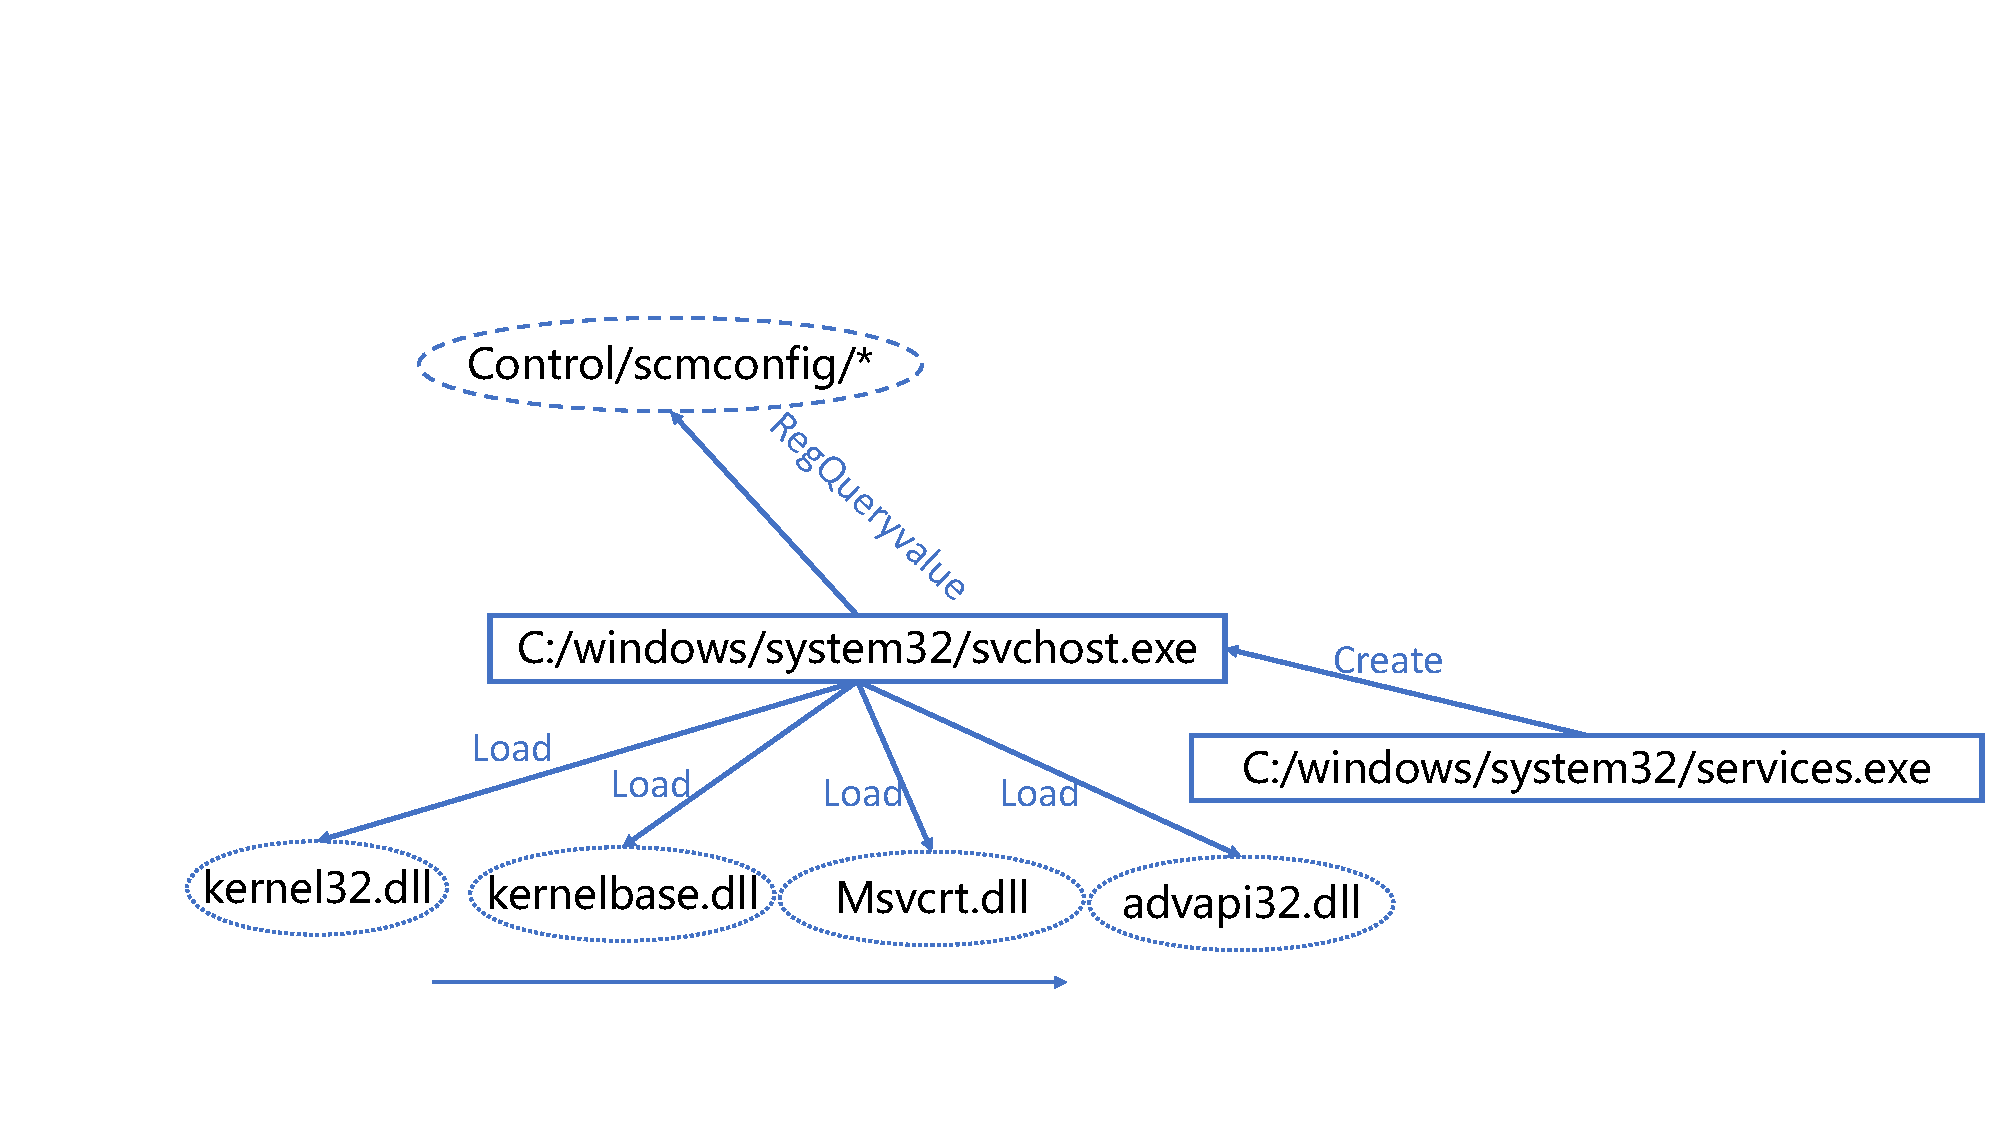
\includegraphics[width=\textwidth]{figs/svchost.pdf}
      \caption{Svchost Constraints in Graph format}
      \label{fig:con-svchost-tree}
  \end{subfigure}
  \hfill
  \begin{subfigure}{.5\textwidth}
      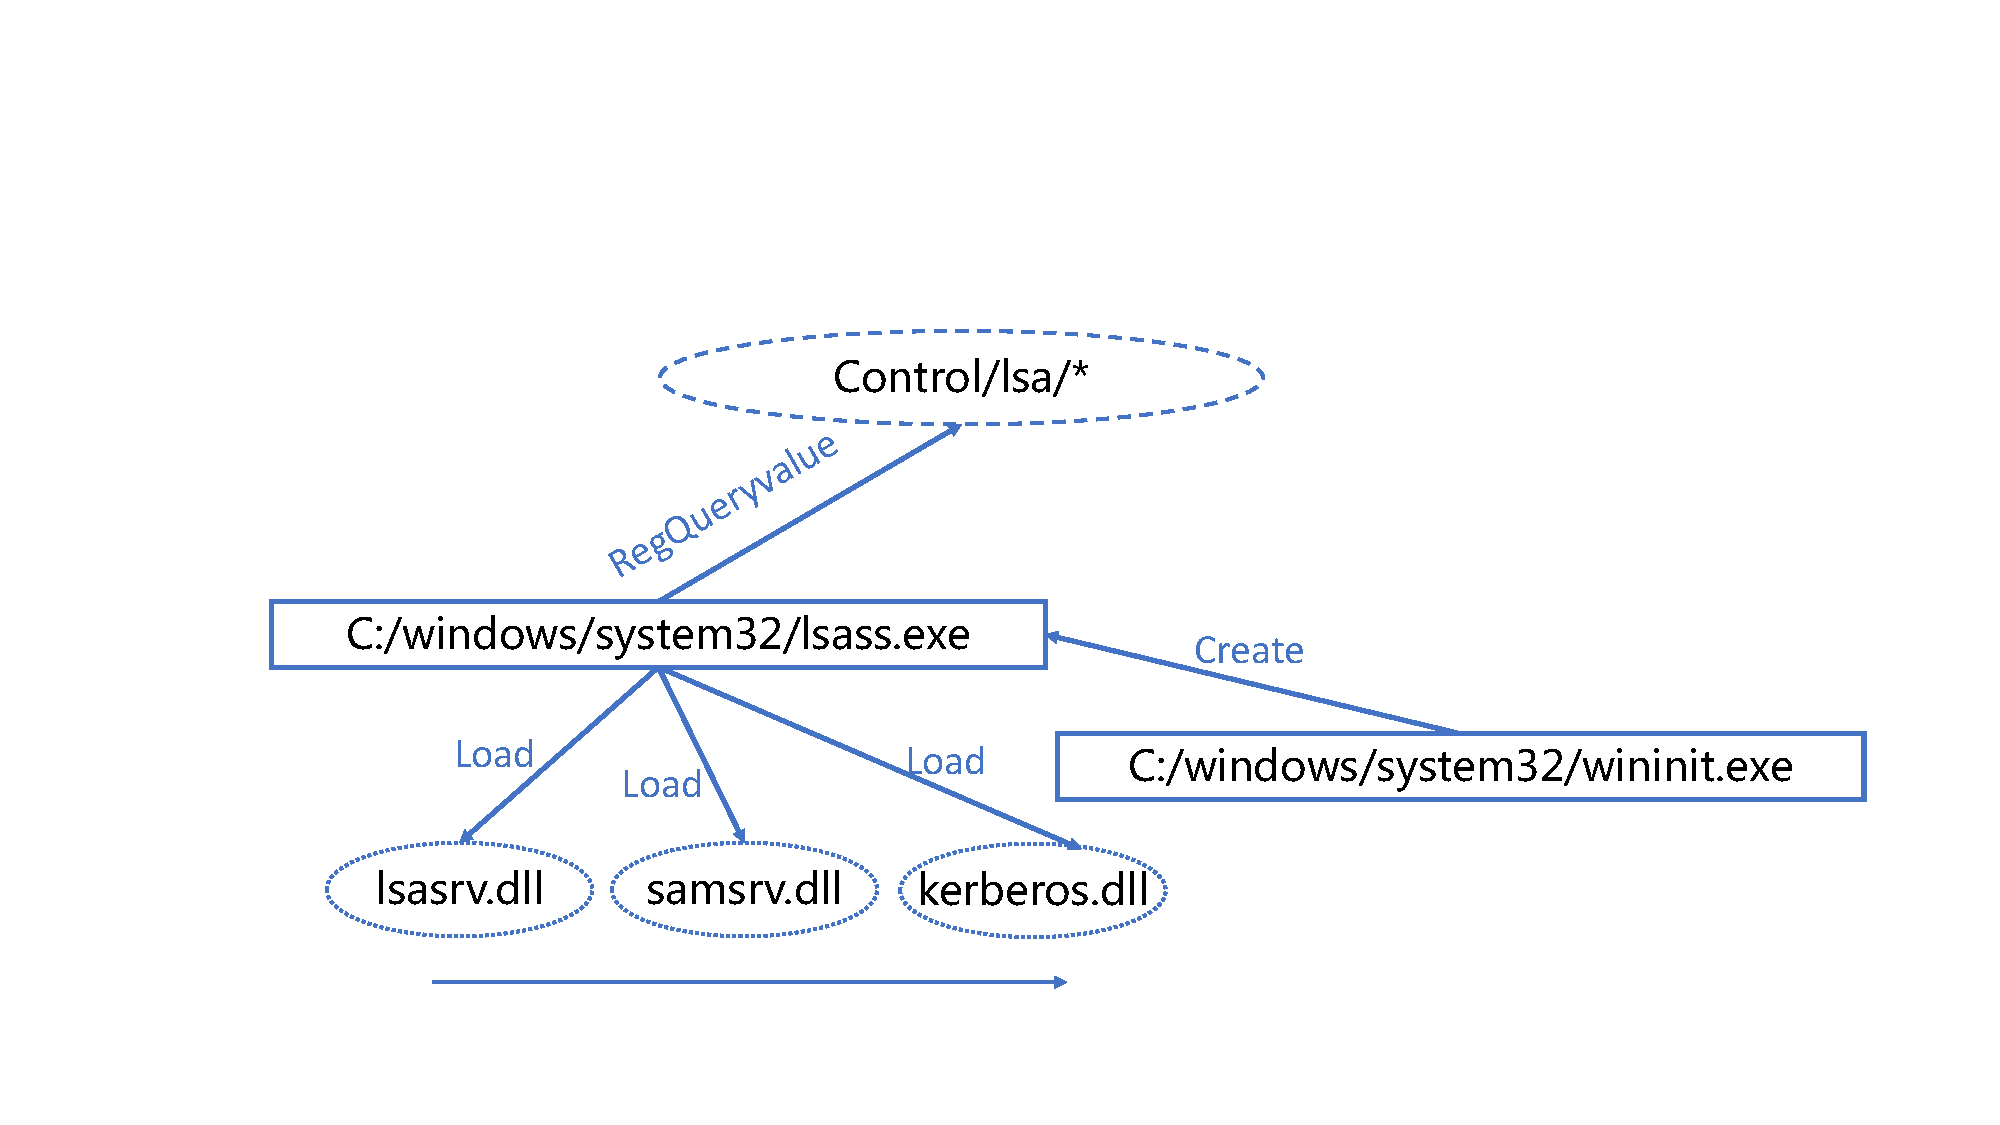
\includegraphics[width=\textwidth]{figs/lsass.pdf}
      \caption{Lsass Constraints in Graph format}
      \label{fig:con-lsass}
  \end{subfigure}
  \caption{Constraint Definition}
  \label{fig:cons-def}
 \end{figure*}


The extraction of system constraints is a pivotal step in our methodology. We begin by categorizing constraints into five types as shown in Figure~\ref{fig:cons-def}.
The Figure~\ref{fig:cons-def} illustrates the constraints of three processes: \textit{svchost.exe}, \textit{lsass.exe}, and \textit{smss.exe}. In Figure~\ref{fig:cons-svchost}, the constraints of \textit{svchost.exe} are shown. There are five types of constraints: execution path, parent process, child process, intrinsic constraints (\textit{svchost.exe} will always load \textit{kernel32.dll} and \textit{advapi32.dll}.), and temporal constraints (\textit{advapi32.dll}, \textit{msvct.dll}, and \textit{kernelbase.dll} must be loaded in the specified sequence).
For certain processes, like \textit{smss.exe}, parent and child processes are optional. The parent process of \textit{smss.exe} can be \textit{system} or \textit{Ntoskml.exe}.
In summary, these constraint relationships can be fully characterized using the AND, OR, and ORDER operators.

By comparing them with the logs gathered in the previous steps, we can validate and extract the first three constraints directly.
However, for intrinsic and temporal constraints, the challenge arises due to real-world logs' vastness. It is impractical to query the LLMs for each log due to memory constraints and its propensity to forget extended conversations. To overcome this, we designed a hybrid method that combines traditional programming techniques with queries to the LLMs to extract these two constraints.

To clearly describe the common items and frequent sequence mining algorithms, we first provide some definitions.
Given a set of log sequences \( \mathcal{D} \), each sequence \( S \in \mathcal{D} \) contains logs \( L \), where each log is a tuple \( L = (s, o, d,t) \) consisting of:
\begin{align*}
    s & : \text{Source process} \\
    o & : \text{Operation} \\
    d & : \text{Destination or object of the operation}\\
    t & : \text{time specifies the timestamp of the event occurrence}
\end{align*}

We want to identify behaviors that are certain to occur in a specific process and in a certain order. 
We begin by mining the logs for common items among different log sequences.   
To speed up common sequence mining, we removed content from sequences that do not include common items when getting common items.
our next step is to use the PrefixSpan algorithm to find common sequences in these logs. 
To obtain the common sequences, rather than frequent sequences, we set the threshold \( \theta =1\) of the PrefixSpan algorithm, indicating that the sequence is certain to occur in the specified order.
(Algorithms are detailed in the Appendix~\ref{alg:fre-common}).
Having established the common items and sequences, we then direct our queries towards the LLMs, focusing specifically on these elements to extract intrinsic and temporal constraints. 
The detailed set of prompts used in this process as shown in Appendix~\ref{prompt-cons-explain}.


\subsubsection{Explanation and Validation}

Furthermore, we request the LLMs to explain its findings, providing insights into these constraints.
Based on the prompt as shown in Appendix~\ref{prompt-cons-explain}, we ask LLMs to explain why this constraint exists, such as why \textit{lsass.exe} must load \textit{lsasrv.dll}, and why \textit{lsass.exe} must load \textit{samsrv.dll} after loading \textit{lsasrv.dll}. 
The LLMs would respond: \textit{lsass.exe} loads \textit{lsasrv.dll} primarily to utilize its code to complete tasks such as authentication and the generation of security tokens. 
\textit{lsass.exe} loads \textit{samsrv.dll} to manage and access the security account database, supporting user authentication and the implementation of local security policies

In addition, due to the potential for hallucinations or misleading results, it is imperative to ensure the accuracy and consistency of LLMs outputs. Due to this challenge, we developed a two-dimensional validation system.

\textbf{Format Validation.}
As a result of this initial step, the model's output adheres to a predefined structure. Using conventional programming methods, deviations are corrected to match the expected format.

\textbf{Factual Validation.}
A more important validation is the factual validation, which is designed to ensure that LLM's final output is accurate and consistent.

\begin{itemize}
    \item Real-world Cross-referencing: LLMs outputs are executed as real-world commands, and their results are cross-checked against real-world logs.
    \item LLMs Multi-session Debates: The LLMs engages in iterative debates in multiple instances. Their goal is to find a consensus on an answer that is both accurate and reliable by verifying each other's responses and reasoning. They cannot reach a consensus on actions that are not entirely correct by having multiple LLMs debate each other. For definitive behaviors, they can eventually come to an agreement. A more detailed description of our approach can be found in the Appendix~\ref{prompt-cross-validation}.
\end{itemize}



\subsection{Threat Detection}
\label{sec:Threat_detection}
An anomaly detection process is based on a multitude of rules derived from the preceding steps. In various attacks, these rules are specifically designed to pinpoint the exact constraints that have been violated. Process masquerading, for example, violates execution pathway and parent-child constraints, whereas process injection violates inherent and temporal constraints more often. This is the basis of our offline process for building individual process profiles. But during online detection, it's possible that some processes might not be on our list.
Our established methodology allows us to profile processes that exist but are not in our knowledge base.

\textbf{Construction Unseen Process Profile.}
The risks and uncertainties associated with incomplete process profiles should be managed and mitigated. Online methods can detect and prevent some attacks caused by incomplete profiles. By using this method, false alarms may be reduced for benign interactions between system entities that were not observed during the construction of the profile.